\documentclass[a4paper, 10pt, twocolumn]{article}
% Sowohl LaTeX als auch pdfLaTeX können benutzt werden, um das Manuskript zu erstellen.

% Bitte öffnen sie diese Datei mit utf8 Zeichenkodierung!!!
\usepackage[utf8]{inputenc}         % Schriftkodierung dieser Datei
% \usepackage[german]{babel}          % für deutsche Dokumente

\usepackage{graphicx}               % optional für Grafiken
\usepackage{tabularx}               % optional für Tabellen
\usepackage{multirow}               % optional für Tabellen
\usepackage{url}                % optional für Internet Links

\usepackage[small,bf]{caption2}     % bitte für Bildunterschriften verwenden
\usepackage{parskip}
\usepackage{titlesec}
\usepackage{amsmath}                % optional für Formeln

\usepackage{tikz}
\usetikzlibrary{arrows}
\usetikzlibrary{decorations.markings}

%\usepackage{showframe}

\titleformat{\section}{\normalfont\large\bfseries}{\thesection}{}{}
\titleformat{\subsection}{\normalfont\large\bfseries}{\thesection}{}{}
\titleformat{\paragraph}{\normalfont\bfseries}{\theparagraph}{}{}
\titlespacing{\section}{0pt}{6pt}{-1pt}
\titlespacing{\subsection}{0pt}{3pt}{-1pt}
\titlespacing{\paragraph}{0pt}{3pt}{-1pt}

\newcolumntype{Y}{>{\centering\arraybackslash}X}    %für Tabellen mit tabularx

% Definition der Seitenränder
\addtolength{\textwidth}{2.1cm}
\addtolength{\topmargin}{-2.4cm}
\addtolength{\oddsidemargin}{-1.1 cm}
\addtolength{\textheight}{4.5cm}
\setlength{\columnsep}{0.7cm}

\pagestyle{empty}                   % weder Kopf- noch Fußzeile auf 1. Seite

\begin{document}

\date{}                                         % kein Datum auf 1. Seite

\title{\vspace{-8mm}\textbf{\large
How Masking Affects Auditory Objects Of Beamformed Sounds}}

% Hier die Namen und Daten der beteiligten Autoren eintragen
\author{
Julian Linke$^1$, Florian Wendt$^2$, Franz Zotter$^2$, Matthias Frank$^2$\\
$^1$ \emph{\small University of Music and Performing Arts, 8010 Graz, Austria, Email: julianweblinke@gmail.com}\\
$^2$ \emph{\small Institute of Electronic Music and Acoustics, Univ. Music and Performing Arts, 8010 Graz, Austria,}\\
\emph{\small Email: \{wendt, zotter, frank\}@iem.at}} \maketitle
\thispagestyle{empty}           % weder Kopf- noch Fußzeile auf Folgeseiten
% Beginn des eigentlichen Manuskripts
\section*{Abstract}
\label{sec:Abstract} 
Sound beams steered into a room modify the balance between wall reflections and direct sound. To some extent, this not only enables lateral auditory object positioning between direct sound and wall reflections, but also in distance, as the level of diffuse reverberation is influenced by directivity. These features made the icosahedral loudspeaker array (IKO), a spherical beamformer, an interesting instrument in electroacoustic music.
In agreement with studies on the precedence effect, previous experiments with the IKO indicated a dependency of the perceived location on how transient the sound is:  Precedence is stronger for transient sounds, therefore these sounds are more strongly determined by the direct sound, hence appear closer to the IKO than continuous sounds.
This contribution investigates how maskers reduce this impact of the precedence effect on transient sounds. For compositions, the experiment of our contribution discusses how far maskers are useful to regain a larger positioning range for transient auditory objects if (a) an audible masker is presented accompanying the transient sound, (b) the direct sound of the transient sound is as quiet to fall below the threshold of hearing, in contrast to the beamforming-emphasized wall reflections.

\section*{Introduction}
\label{sec:Introduction} 

\section*{Experiment on Localization}
\label{sec:Experiment on Localization} 

\subsection*{Method}
\label{sec:Method}

\begin{figure}[ht]
\centering
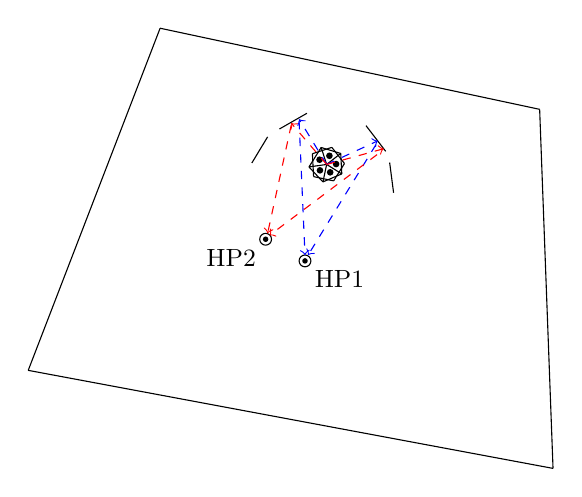
\begin{tikzpicture}[scale = 0.5]
% KOORDINATEN
% \coordinate[label=below:$\texttt{Ursprung}$] (Ursprung) at (0,0);
\coordinate (POSIKO) at (.7,1.7);
\coordinate[label=below right:$\text{\small HP1}$]  (HP1) at (.15,-.75);
\coordinate[label=below left:$\text{\small HP2}$]  (HP2) at (-.85,-.2);

% Raum
\coordinate (LO) at (-3.53,5.16);
\coordinate (RO) at (6.11,3.10);
\coordinate (LU) at (-6.88,-3.53);
\coordinate (RU) at (6.45,-6.02);
% Reflektor 1
\coordinate (R1U) at (-1.2,1.737);
\coordinate (R1O) at (-.8,2.4);
% Reflektor 2
\coordinate (R2U) at (-.5,2.6);
\coordinate (R2O) at (0.2,3);
% Reflektor 3
\coordinate (R3U) at (2.2,2.033);
\coordinate (R3O) at (1.7,2.685);
% Reflektor 4
\coordinate (R4O) at (2.3,1.749);
\coordinate (R4U) at (2.4,.981);
% IKO
\coordinate (IKO1) at (.25126,1.6369);
\coordinate (IKO2) at (0.60578,1.2567);
\coordinate (IKO3) at (1.0843,1.4599);
\coordinate (IKO4) at (1.0571,1.979 );
\coordinate (IKO5) at (0.55997,2.131);
\coordinate (IKO6) at (0.36858,1.3909);
\coordinate (IKO7) at (0.87706,1.2829);
\coordinate (IKO8) at (1.1525,1.7237);
\coordinate (IKO9) at ( 0.83249,2.1334);
\coordinate (IKO10) at ( 0.3381,1.9727);

% ZEICHNEN
\draw (R1U) -- (R1O);
\draw (R2U) -- (R2O);
\draw (R3U) -- (R3O);
\draw (R4U) -- (R4O);

\draw (IKO6) -- (IKO7);
\draw (IKO7) -- (IKO8);
\draw (IKO8) -- (IKO9);
\draw (IKO9) -- (IKO10);
\draw (IKO10) -- (IKO6);

\draw (IKO1) -- (IKO2);
\draw (IKO2) -- (IKO3);
\draw (IKO3) -- (IKO4);
\draw (IKO4) -- (IKO5);
\draw (IKO5) -- (IKO1);

\draw (POSIKO) -- (IKO1);
\draw (POSIKO) -- (IKO2);
\draw (POSIKO) -- (IKO3);
\draw (POSIKO) -- (IKO4);
\draw (POSIKO) -- (IKO5);

\draw (LO) -- (RO);
\draw (RO) -- (RU);
\draw (RU) -- (LU);
\draw (LU) -- (LO);

% \draw[help lines] (-3,-3) grid (3,3);
\draw (HP1) circle [radius=1.5mm] ;
\draw (HP2) circle [radius=1.5mm] ;

% \fill (Ursprung) circle (2pt);
\fill (POSIKO) circle (1pt);
\fill (.79,1.5) circle (2.4pt);
\fill (.94,1.71) circle (2.4pt);
\fill (.77,1.92) circle (2.4pt);
\fill (.52,1.82) circle (2.4pt);
\fill (.53,1.55) circle (2.4pt);
\fill (HP1) circle (2pt);
\fill (HP2) circle (2pt);

% Schallstrahl links HP1
% \draw[blue,dashed,->,-triangle 90,fill=blue] (POSIKO) -- (0,2.85);
\draw[blue,dashed,->] (POSIKO) -- (0,2.85);
\draw[blue,dashed,->] (0,2.8) -- (.15,-.6);
% Schallstrahl rechts HP1
\draw[blue,dashed,->] (POSIKO) -- (2,2.3);
\draw[blue,dashed,->] (1.95,2.20) -- (.23,-.6);
% Schallstrahl links HP2
\draw[red,dashed,->] (POSIKO) -- (-.2,2.75);
\draw[red,dashed,->] (-.2,2.7) -- (-.8,-.05);
% Schallstrahl rechts HP2
\draw[red,dashed,->] (POSIKO) -- (2.15,2.1);
\draw[red,dashed,->] (1.98,1.95) -- (-0.75,-.1);
\end{tikzpicture}
\caption{Diagram of the CUBE for the listening experiment. The hearing position 1 (HP1) was directly in front of the IKO with a distance of $2.5m$. The hearing position 2 (HP2) was further ahead and approximatley 1 meter apart. The reflectors were placed symmetrically around the IKO. The noise and the beamformed sounds were presented by the IKO.}
\end{figure} %% include figure of example

\subsection*{Results}
\label{sec:Results}

\begin{figure}[ht]
	\centering
	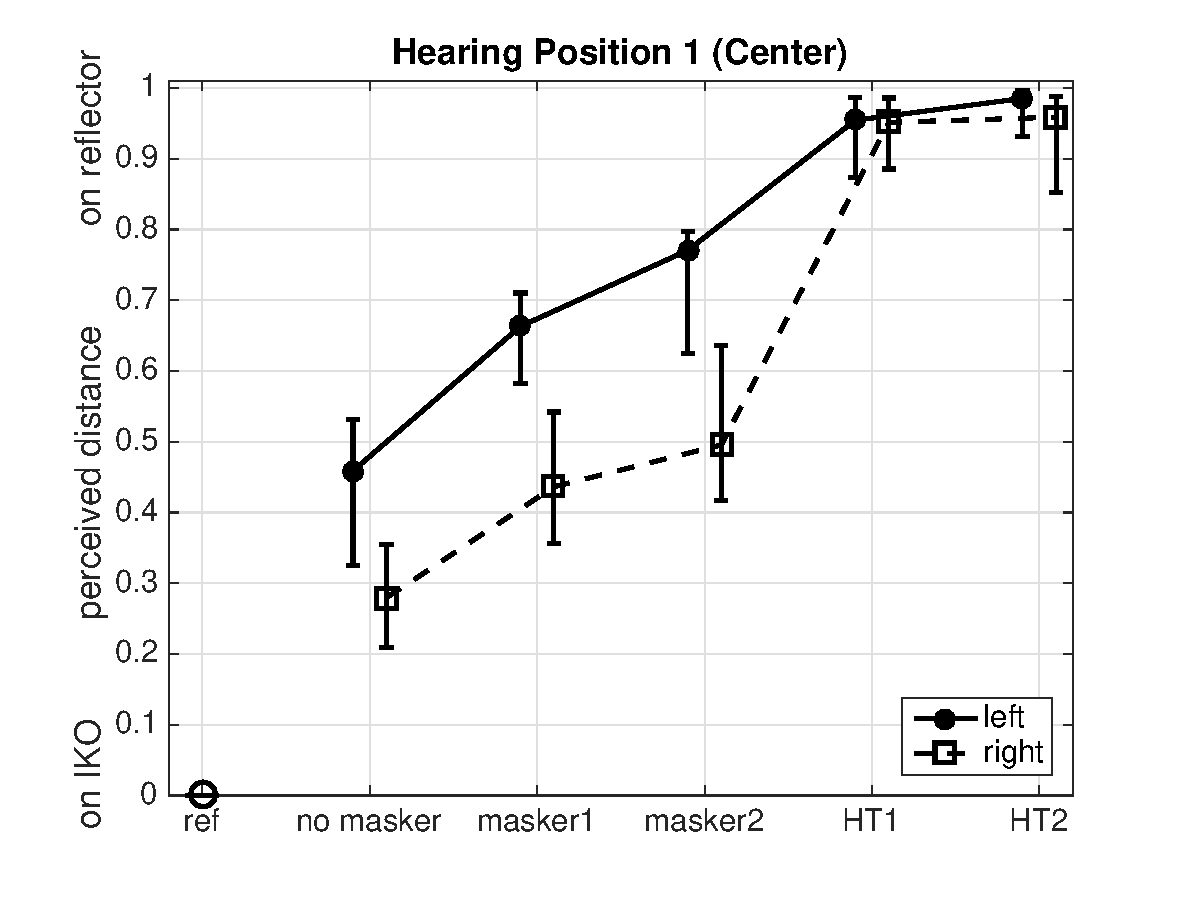
\includegraphics[scale=0.5]{./figures/center.eps}
	\caption{results center}
\end{figure}

\begin{figure}[ht]
	\centering
	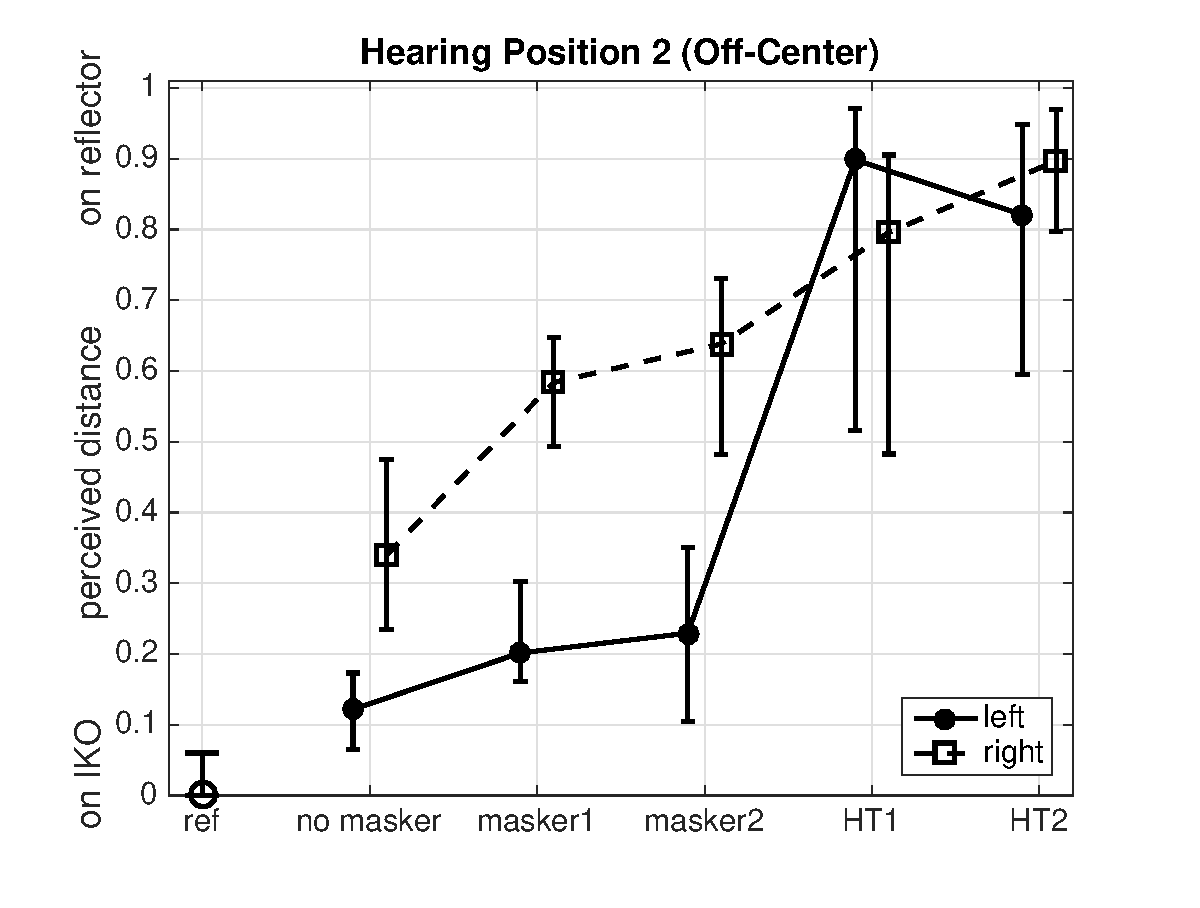
\includegraphics[scale=0.5]{./figures/offcenter.eps}
	\caption{results off-center}
\end{figure}

\begin{thebibliography}{5}
\bibitem{ArticleReference}
Schall, A.: How to write a manuscript. Acta Acustica united with
Acustica 90 (2004), 2203-2503
\bibitem{BookReference}
Klang, B.: Akustik im Überblick. Schall und Rauch Verlag, Stadt,
2010
\bibitem{URLReference}
DAGA 2018 Homepage, URL:\\
\url{http://www.2018.daga-tagung.de//}
\bibitem{PDFCreator}
PDFCreator, URL:\\
\url{http://sourceforge.net/projects/pdfcreator}
\bibitem{Ghostware}
Free software Ghostview and Ghostscript, URL:\\
\url{http://www.cs.wisc.edu/~ghost/}
\end{thebibliography}
\end{document}
